


\chapter{Evaluation of Minimalist Prover\label{ch:proverEvaluation}}
%-----------------------------------------------------------------------------
The evaluation of our minimalist prover orbits three fundamental questions: first, does our prover succeed in verifying programs; second, are our heuristics effective at increasing the usefulness of the prover; and third, does the data gathered by our prover expose any interesting properties of the VCs that arise from well-engineered programs.

The first and second question are explored by considering a series of verification benchmarks.  In Section \ref{canProve} we present each benchmark, then explore the effectiveness of the automated prover when applied to that benchmark.  Following that, in Section \ref{heuristicsEval}, we use those same benchmarks to explore how our various heuristics impact the effectiveness of the prover.  Finally, the third question is addressed in Section \ref{proverEvalConclusion}, where we provide some observations and conclusions based on the collected data.

This chapter focuses on the specifications and realizations of the benchmarks, with discussion of relevant mathematics forming the basis of Chapter \ref{ch:mathEvaluation}.  We will generally present only enough of each specification and realization to motivate our discussion, but the full specifications of each benchmark and any associated datastructures can be found in Appendix \ref{apx:spec} and full realizations in Appendix \ref{apx:real}.  Full listings of the proofs generated as solutions to the benchmarks in this chapter are available in Appendix \ref{apx:proofs}.

While the usability of our prover and its application in educational settings is not a core part of this thesis, we take this opportunity to note that our minimalistic prover has provided the backbone of our educational web-interface for three years now, and point the interested reader at \cite{cook2012specification} or \cite{sitaraman2009engaging} for examples of research where our prover is applied in educational settings.


%-----------------------------------------------------------------------------
\section{Description of Metrics}
%-----------------------------------------------------------------------------
For this chapter we focus on four primary metrics for exploring the effectiveness of the prover and the difficulty of the VCs.  These are:

\begin{itemize}
	\item \textbf{VCs proved.}  The number of VCs that were successfully dispatched by the prover.  Since the proof space is quite large, the prover often runs with a set timeout, after which it gives up, so in reality this metric refers to the number of VCs that were proved within the timeout.  Throughout this chapter, the timeout was set at 20 seconds.
	\item \textbf{Real time.}  The amount of time required to dispatch the VC, generally measured in milliseconds.  Because this metric can vary depending on a number of variables, we will generally use the median of five repeated trials.
	\item \textbf{Proof steps.}  The number of relevant steps taken by the prover.  One of the features of the prover is to prune steps that did not impact the final result.
	\item \textbf{Search steps.}  A subset of the overall proof steps including only those steps taken during the ``consequent exploration'' phase described in Section \ref{consequentExploration}, and not including those consequent steps that are ``obvious'', namely: replacing a consequent that matches a given with \texttt{true}, replacing a consequent that is a symmetric equality with \texttt{true}, and eliminating a conjunct that is \texttt{true}.  Intuitively this metric refers to the number of steps that were blind exploration of the proof space and which may have to be backtracked over, rather than deterministic steps over which we do not backtrack.
\end{itemize}


%-----------------------------------------------------------------------------
\section{Benchmark Solutions\label{canProve}}
%-----------------------------------------------------------------------------

%-----------------------------------------------------------------------------
	\subsection{VSTTE Benchmarks}
%-----------------------------------------------------------------------------
In 2010, members of the RSRG at Clemson and The Ohio State University published a set of incremental verification benchmarks at the Verified Software: Tools, Theories, and Experiments workshopVSTTE\cite{Benchmarks}.  These benchmarks were intended to provide a basis for experimentation and discussion between verification efforts.  In \cite{hartonDissertation}, the author presents a selection of these benchmarks implemented in RESOLVE in order to demonstrate the VC-generation capabilities of the RESOLVE compiler.  We mirror that methodology in this section, presenting a selection of the VSTTE benchmarks, including several that are borrowed or adapted from \cite{hartonDissertation}, before applying our minimalist prover to them and presenting resulting data.
	%-----------------------------------------------------------------------------
		\subsubsection{Benchmark 1: Adding and Multiplying Integers}	%-----------------------------------------------------------------------------

\paragraph{Problem Statement}Verify an operation that adds two numbers by repeated incrementing. Verify an operation that multiplies two numbers by repeated addition, using the first operation to do the addition. Make one algorithm iterative, the other recursive.\footnote{This and all other problem statements quote directly from \cite{Benchmarks}.}

\paragraph{Solution Discussion}In Listing \ref{lst:integerAddMultSpec} we present specifications of integer addition and multiplication operations in RESOLVE.  Each of these operations is specified to work ``in place'', transforming the first parameter (which is also used as one of the inputs) into the final solution.

\lstinputlisting[float=h,language=resolve,caption={The specification of \texttt{Adding\_Capabilitiy} and \texttt{Multiplying\_Capability}\label{lst:integerAddMultSpec}}]{proverEval/examples/IntegerPlusTimesSpecs.en}

Each specifies that its second parameter must be positive---dealing correctly with the presence of negative numbers adds a surprising amount of implementation complexity for a language like RESOLVE that strives to correctly reason about bounded integers, since the maximum and minimum integer are generally not symmetrical.  Note, however, that we lose no generality---a more general addition or multiplication function could be specified and wrapped around the ones presented in this section, transforming any addition or multiplication task into a finite subset of tasks that could computed correctly by these implementations.

We experimented both with an iterative and recursive implementation of \texttt{Adding\_Capability}.  We present the rescursive implementation in Listing \ref{lst:addImpl}.  The iterative implementation is available in Appendix \ref{apx:spec}.

\lstinputlisting[float=h,language=resolve,caption={A recursive implementation of \texttt{Adding\_Capabilitiy}\label{lst:addImpl}}]{proverEval/examples/Recursive_Add_to_Realiz.rb}

Our implementation of \texttt{Multiplying\_Capabilitiy} is iterative and presented in Listing \ref{lst:multImpl}.

\lstinputlisting[float=h,language=resolve,caption={An iterative implementation of \texttt{Multiplying\_Capabilitiy}\label{lst:multImpl}}]{proverEval/examples/Iterative_Multiply_into_Realiz.rb}

\begin{sloppypar}
Integers are partially built-in to RESOLVE, which makes using one enhancement to \texttt{Integer\_Template} from another fairly unweildy, which is why we do not use \texttt{Adding\_Capability} to implement \texttt{Multiplying\_Capability} as requested by the benchmark, but rather the normal integer \texttt{+}.  We note, however, that \texttt{+} is drawn from \texttt{Integer\_Template} as a normal specification and thus presents the same verification challenges (that is: reasoning about it is not built in).
\end{sloppypar}

\paragraph{Results}Each of our three implementations is fully verifiable.  The results of those verifications, with associated metrics is presented in Figure \ref{fig:addMultResults}.

\begin{figure}
	\centering
	\begin{subfigure}[b]{0.45\textwidth}
		\centering
		\begin{tabular}{lrrrr}
			\toprule
				& Time (ms)	& $\sigma$& Steps & Search \\
			\midrule
			VC 0\_1	& 5560		& 182	& 5	& 0     \\
			VC 0\_2	& 3456		& 280	& 5	& 0     \\
			VC 0\_3	& 565		& 78	& 10	& 0     \\
			VC 0\_4	& 834		& 197	& 9	& 0     \\
			VC 0\_5	& 3873		& 219	& 6	& 0     \\
			VC 0\_6	& 613		& 101	& 8	& 0     \\
			VC 0\_7	& 591		& 106	& 5	& 0     \\
			VC 1\_1	& 5020		& 286	& 9	& 0     \\
			\bottomrule
		\end{tabular}
		\caption{Iterative \texttt{Adding\_Capabilitiy} results\label{fig:iterAddResults}}
	\end{subfigure}
	\qquad
	\begin{subfigure}[b]{0.45\textwidth}
		\centering
		\begin{tabular}{lrrrr}
			\toprule
				& Time (ms)	& $\sigma$& Steps & Search \\
			\midrule
			VC 0\_1	& 2549		& 124	& 9	& 0     \\
			VC 0\_2	& 1244		& 221	& 9	& 0     \\
			VC 0\_3	& 977		& 177	& 5	& 0     \\
			VC 0\_4	& 1379		& 222	& 6	& 0     \\
			VC 0\_5	& 1118		& 159	& 6	& 0     \\
			VC 0\_6	& 757		& 82	& 8	& 0     \\
			VC 0\_7	& 1113		& 178	& 5	& 0     \\
			VC 1\_1	& 379		& 76	& 8	& 0     \\
			\bottomrule
		\end{tabular}
		\caption{Recursive \texttt{Adding\_Capabilitiy} results\label{fig:recAddResults}}
	\end{subfigure}

	\vspace{2em}
	\begin{subfigure}[b]{0.6\textwidth}
		\centering
		\begin{tabular}{lrrrr}
			\toprule
				& Time (ms)	& $\sigma$& Steps & Search \\
			\midrule
			VC 0\_1	& 6264		& 195	& 7	& 0     \\
			VC 0\_2	& 3484		& 365	& 5	& 0     \\
			VC 0\_3	& 3495		& 182	& 7	& 2     \\
			VC 0\_4	& 393		& 149	& 7	& 0     \\
			VC 0\_5	& 333		& 53	& 5	& 0     \\
			VC 1\_1	& 5917		& 124	& 8	& 0     \\
			\bottomrule
		\end{tabular}
		\caption{Iterative \texttt{Multiplying\_Capabilitiy} results\label{fig:iterMultResults}}
	\end{subfigure}
  \caption{Results from verification of Benchmark 1 solutions\label{fig:addMultResults}}
\end{figure}


%-----------------------------------------------------------------------------
		\subsubsection{Benchmark 2: Benchmark 2: Binary Search an Array}	%-----------------------------------------------------------------------------

\paragraph{Problem Statement}Verify an operation that uses binary search to find a given entry in an array of entries that are in sorted order.

\paragraph{Solution Discussion}In Listing \ref{lst:searchSpec} we present a specification of a searching operation on an array.  The operation takes as its input an entry and an array in sorted order, then uses a parameterizable comparison function, \texttt{LEQ}, to search the array.

\lstinputlisting[float=h,language=resolve,caption={The specification of \texttt{Searching\_Capabilitiy}\label{lst:searchSpec}}]{proverEval/examples/Search_Capability.en}

The \emph{requires} clause of the operation uses higher-order definitions to establish that the array is in order---i.e., that it is \emph{conformal} with the given comparator.  The \emph{ensures} clause states that the operation will return \texttt{true} if and only if the given entry exists between the lower and upper bound of the array.  The details of these higher-order definitions are explored more fully in Chapter \ref{ch:mathEvaluation}.

An implementation for this operation is provided in Listing \ref{lst:searchImpl}.

\lstinputlisting[float=h,language=resolve,caption={An implementation of \texttt{Searching\_Capabilitiy}\label{lst:searchImpl}}]{proverEval/examples/Bin_Search_Realiz.rb}

The realization takes a function, \texttt{Are\_Ordered()} which provides a programmatic way of establishing \texttt{LEQ}.  From there, the implementation is the usual straightforward binary search implementation.  Note that when calculating the new mid, we first take the difference, then divide, avoiding the overflow problem exposed in \cite{blochBinarySearch}.

While we provide syntactic sugar for array operations, they are supported by an ordinary component that provides specifications for all array operations, a snippet of which is provided in Listing \ref{lst:arraySpec}.

\lstinputlisting[float=h,language=resolve,caption={A snippet of the specification of arrays\label{lst:arraySpec}}]{proverEval/examples/Static_Array_Template.co}

\paragraph{Results} Of the 45 VCs generated by this example, we are able to mechanically verify 39.  These result are summarized in Figure \ref{fig:binSearchResults}.

\begin{figure}
	\centering
	\begin{tabular}{lrrrr}
		\toprule
			& Time (ms)	& $\sigma$& Steps & Search \\
		\midrule
		VC 0\_1	& 1411		& 174 	& 6 	& 1     \\
		VC 0\_2	& 819		& 161	& 5 	& 0     \\
		VC 0\_3	& 573		& 107	& 5 	& 0     \\
		VC 1\_1	& 2523		& 249	& 8 	& 0     \\
		VC 1\_2	& 1607		& 148	& 5	& 0     \\
		VC 1\_3	& 1318		& 111	& 5 	& 0     \\
		VC 1\_4	& 792		& 155	& 5 	& 0     \\
		VC 1\_5	& 6438		& 261	& 10	& 3     \\
		VC 1\_6	& 2401		& 302	& 9 	& 1     \\
		VC 1\_7	& 6838 		& 178	& 10	& 3     \\
		VC 1\_8	& 2430 		& 188	& 9	& 1     \\
		VC 1\_9	& \multicolumn{4}{c}{Not Proved}        \\
		VC 1\_10 & 2108		& 191	& 7 	& 1     \\
		VC 1\_11 & 2097		& 305	& 5 	& 0     \\
		VC 1\_12 & \multicolumn{4}{c}{Not Proved}       \\
		VC 1\_13 & 3259		& 309	& 9	& 3     \\
		VC 2\_1	& 1637		& 116	& 8 	& 0     \\
		VC 2\_2	& 1346		& 98	& 5	& 0     \\
		VC 2\_3	& 1361		& 99	& 5 	& 0     \\
		VC 2\_4	& 595		& 35	& 5 	& 0     \\
		VC 2\_5	& 5816		& 247	& 10	& 3     \\
		VC 2\_6	& 2414		& 121	& 9 	& 1     \\
		VC 2\_7	& 6465 		& 338	& 10	& 3     \\
		\bottomrule
	\end{tabular}
	\quad
	\begin{tabular}{lrrrr}
		\toprule
			& Time (ms)	& $\sigma$& Steps & Search \\
		\midrule
		VC 2\_8	& 2813 		& 187	& 9	& 1     \\
		VC 2\_9	& \multicolumn{4}{c}{Not Proved}        \\
		VC 2\_10 & 2923		& 393	& 11	& 4     \\
		VC 2\_11 & 2369		& 260	& 5 	& 0     \\
		VC 2\_12 & \multicolumn{4}{c}{Not Proved}       \\
		VC 2\_13 & 11229	& 204	& 8	& 3     \\
		VC 3\_1	& 1715		& 124	& 8 	& 0     \\
		VC 3\_2	& 1322		& 139	& 5	& 0     \\
		VC 3\_3	& 1242		& 140	& 5 	& 0     \\
		VC 3\_4	& 630		& 64	& 5 	& 0     \\
		VC 3\_5	& 6095		& 151	& 10	& 3     \\
		VC 3\_6	& 2540		& 306	& 9	& 1     \\
		VC 3\_7	& 6388 		& 335	& 10	& 3     \\
		VC 3\_8	& 2730 		& 230	& 9	& 1     \\
		VC 3\_9	& \multicolumn{4}{c}{Not Proved}        \\
		VC 3\_10 & 2386		& 228	& 5 	& 0     \\
		VC 3\_11 & 2785		& 300	& 10	& 2     \\
		VC 3\_12 & \multicolumn{4}{c}{Not Proved}       \\
		VC 3\_13 & 18032	& 273	& 9	& 2     \\
		VC 4\_1	& 2474		& 70	& 9 	& 3     \\
		VC 4\_2	& 787		& 129	& 5	& 0     \\
		VC 4\_3	& 813		& 71	& 5 	& 0     \\
		\bottomrule
	\end{tabular}
	\caption{Binary search \texttt{Searching\_Capabilitiy} results\label{fig:binSearchResults}}
\end{figure}

The six VCs that are not mechanically verified represent a failure not of the prover---but rather of RESOLVE's underlying syntax.  Because at this time RESOLVE does not permit the application of an arbitrary expression (as opposed to a named function), we are unable to formulate the required theorems to prove these VCs.

We now present a manual proof of a representative one of these VCs by hand and argue that once this syntactic problem is resolved, our minimalist prover will be easily able to dispatch the VC.

Consider the VC in Listing \ref{lst:brokenVC} corresponding to the inductive case of the while loop's maintaining clause.  Irrelevant givens have been ommited for brevity.

\lstinputlisting[float=h,language=resolve,caption={A problematic VC\label{lst:brokenVC}}]{proverEval/examples/BrokenVC.asrt}

Let us now proceed as the mechanical prover would.  We first replace instances of \texttt{A''} with \texttt{A}, resulting in these givens:

\begin{verbatim}
A' = lambda ( j : Z ).(
	{{midVal'' if j = (low'  + ((high'  - low')  / 2))
	  A(j) otherwise}}) and
A((low'  + ((high'  - low')  / 2))) = key)
\end{verbatim}

We now replace \texttt{A'} with its full expansion in the goal, resulting in this new goal:

\begin{verbatim}
lambda ( j : Z ).(
	{{key if j = (low'  + ((high'  - low')  / 2))
	  lambda ( j : Z ).(
		{{midVal'' if j = (low'  + ((high'  - low')  / 2))
	  	A(j) otherwise}}(j) otherwise}})
= A
\end{verbatim}

Finally, we replace instances of \texttt{key} with its expansion, resulting in this new goal (we change the internal lambda's variable to \texttt{k} for clarity, though the prover does not have to deal with this complication):

\begin{verbatim}
lambda ( j : Z ).(
	{{A((low'  + ((high'  - low')  / 2))) 
		if j = (low'  + ((high'  - low')  / 2))
	  lambda ( k : Z ).(
		{{midVal'' if k = (low'  + ((high'  - low')  / 2))
	  	A(k) otherwise}})(j) otherwise}})
= A
\end{verbatim}

At this point we are able to apply the theorem given in Listing \ref{lst:lambdaThm} (note that it applies a function-valued expression when it evaluates a lambda expression at \texttt{x} and therefore cannot be represented in our current syntax).

\begin{lstlisting}[float=h,language=resolve,caption={A useful theorem about lambda expressions\label{lst:lambdaThm}}]
Theorem Shadowed_Function_Piece:
	For all T, R : MType,
	For all t : T,
	For all r : R,
	For all f : T -> R,
		f = lambda (x : T).(
			{{f(x) if x = t;
			  lambda (y : Z).(
				{{r if y = t;
				  f(y) otherwise}})(x) otherwise}});
\end{lstlisting}

We are then left with simply \texttt{A~=~A}, at which point the remainder of the proof is trivial.  Each of these six VCs has a similar straightforward proof.

\FloatBarrier
%-----------------------------------------------------------------------------
		\subsubsection{Benchmark 3: Sorting a Queue}	%-----------------------------------------------------------------------------

\paragraph{Problem Statement}Specify a user-defined FIFO queue ADT that is generic (i.e., parameterized by the type of entries in a queue). Verify an operation that uses this component to sort the entries in a queue into some client-defined order.

\paragraph{Solution Discussion}In Listing \ref{lst:sortingSpec} we present a specification of a queue sorting enhancement.  As with Benchmark 2, it takes as a parameter a client-provided definition to define the sorted order, \texttt{LEQV}.  It uses two higher-order definitions \texttt{Is\_Coformal\_With()} and \texttt{Is\_Permutation()} to ensure that the final queue is ordered according to \texttt{LEQV} and contains the same elements as those original provided, respectively.

\lstinputlisting[float=h,language=resolve,caption={The specification of \texttt{Sorting\_Capability}\label{lst:sortingSpec}}]{proverEval/examples/Sorting_Capability.en}

A straightforward selection sort realization is provided in Listing \ref{lst:sortingImpl}.

\lstinputlisting[float=h,language=resolve,caption={A selection sort realization of \texttt{Sorting\_Capabilitiy}\label{lst:sortingImpl}}]{proverEval/examples/Selection_Sort_Realization.rb}

Again, as in Benchmark 2, we take a client-provided operation, \texttt{Compare()}, that implements \texttt{LEQV}, and use it to implement our \texttt{Remove\_Min()} sub-operation.  The \texttt{One()} and \texttt{Two()} procedures simply provide a way of getting the programmatic values \texttt{1} and \texttt{2} using a normal specification.

\paragraph{Results}This implementation is fully verifiable.  The results of that verifications, with associated metrics, is presented in Figure \ref{fig:sortingResults}.  Based on our literature review, we believe that RESOLVE is the only verification effort with a generic, automatically-verifiable selection sort\footnote{The RESOLVE group at The Ohio State University has their own version of this automatically-verifiable selection sort.  We note, however, that their system takes advantage of a specialized decision procedure for reasoning about strings, whereas our solution uses only our generalized minimalist prover.}

\begin{figure}
	\centering
	\begin{tabular}{lrrrr}
		\toprule
			& Time (ms)	& $\sigma$& Steps & Search \\
		\midrule
		VC 0\_1	& 1344		& 242 	& 6 	& 0     \\
		VC 0\_2	& 479		& 73	& 5 	& 0     \\
		VC 0\_3	& 912		& 56	& 5 	& 0     \\
		VC 0\_4	& 1305		& 198	& 6 	& 1     \\
		VC 0\_5	& 2762		& 300	& 8	& 0     \\
		VC 0\_6	& 3128		& 372	& 9 	& 3     \\
		VC 0\_7	& 1513		& 271	& 8 	& 0     \\
		VC 0\_8	& 1710		& 136	& 10	& 1     \\
		VC 0\_9	& 2219		& 166	& 9 	& 3     \\
		VC 1\_1	& 501 		& 100	& 5 	& 0     \\
		VC 1\_2	& 1012 		& 165	& 10	& 1     \\
		VC 2\_1	& 806 		& 136	& 5 	& 0     \\
		VC 2\_2	& 1918		& 237	& 8 	& 0     \\
		VC 2\_3	& 1781		& 197	& 5 	& 0     \\
		VC 2\_4	& 1620		& 284	& 6 	& 1     \\
		VC 2\_5	& 3021		& 387	& 14	& 0     \\
		\bottomrule
	\end{tabular}
	\qquad
	\begin{tabular}{lrrrr}
		\toprule
			& Time (ms)	& $\sigma$& Steps & Search \\
		\midrule
		VC 2\_6	& 4441		& 278	& 12	& 3     \\
		VC 2\_7	& 1919		& 108	& 10	& 2     \\
		VC 2\_8	& 1843		& 139	& 7 	& 0     \\
		VC 3\_1	& 819 		& 141	& 5 	& 0     \\
		VC 3\_2	& 1896		& 213	& 8 	& 0     \\
		VC 3\_3	& 1642		& 124	& 5 	& 0     \\
		VC 3\_4	& 1493		& 197	& 6 	& 1     \\
		VC 3\_5	& 2965		& 239	& 14	& 0     \\
		VC 3\_6	& 4202		& 200	& 10	& 1     \\
		VC 3\_7	& 1897		& 194	& 10	& 2     \\
		VC 3\_8	& 1863		& 165	& 7 	& 0     \\
		VC 4\_1	& 838 		& 139	& 5 	& 0     \\
		VC 4\_2	& 2939		& 150	& 12	& 0     \\
		VC 4\_3	& 1132		& 189	& 5 	& 0     \\
		VC 4\_4	& 3056		& 262	& 18	& 3     \\
		\bottomrule
	\end{tabular}
	\caption{Selection sort \texttt{Sorting\_Capabilitiy} results\label{fig:sortingResults}}
\end{figure}

\FloatBarrier
%-----------------------------------------------------------------------------
	\subsection{Other Benchmarks}
%-----------------------------------------------------------------------------

%-----------------------------------------------------------------------------
		\subsubsection{Benchmark 4: Reversing a Queue}	%-----------------------------------------------------------------------------

\paragraph{Problem Statement}Specify a user-defined FIFO queue ADT that is generic (i.e., parameterized by the type of entries in a queue). Verify an operation that reverses the entries in a given queue.

\paragraph{Solution Discussion}In Listing \ref{lst:flippingSpec} we present a specification of a queue reversing enhancement called \texttt{Flipping\_Capability}.  A recursive solution follows in Listing \ref{lst:flippingImpl}.


\lstinputlisting[float=h,language=resolve,caption={The specification of \texttt{Flipping\_Capabilitiy}\label{lst:flippingSpec}}]{proverEval/examples/Flipping_Capability.en}

\lstinputlisting[float=h,language=resolve,caption={A recursive realization of \texttt{Flipping\_Capabilitiy}\label{lst:flippingImpl}}]{proverEval/examples/Recursive_Flipping_Realiz.rb}

\paragraph{Results}This implementation is fully verifiable.  The results of that verifications, with associated metrics, is presented in Figure \ref{fig:flippingResults}.

\begin{figure}
	\centering
	\begin{tabular}{lrrrr}
		\toprule
			& Time (ms)	& $\sigma$& Steps & Search \\
		\midrule
		VC 0\_1	& 1520		& 141	& 5 	& 0     \\
		VC 0\_2	& 3118		& 295	& 7 	& 0     \\
		VC 0\_3	& 2741		& 222	& 8 	& 0     \\
		VC 0\_4	& 2174		& 170	& 9 	& 2     \\
		VC 1\_1	& 366		& 83	& 10	& 0     \\
		\bottomrule
	\end{tabular}
	\caption{Recursive \texttt{Flipping\_Capabilitiy} results\label{fig:flippingResults}}
\end{figure}


%-----------------------------------------------------------------------------
		\subsubsection{Benchmark 5: Array Realization of Stack}	%-----------------------------------------------------------------------------

\paragraph{Problem Statement}Specify a user-defined LIFO stack ADT that is generic (i.e., parameterized by the type of entries in a queue). Verify an implementation of that array.

\paragraph{Solution Discussion}Listing \ref{lst:stackSpec} gives RESOLVE's specification for a stack in the context of a \texttt{Stack\_Template}, which is generic and bounded.

\lstinputlisting[float=h,language=resolve,caption={The specification of \texttt{Stack}\label{lst:stackSpec}}]{proverEval/examples/Stack_Template.co}

We implement this specification on top of an array, which, as in Benchmark 2, is a first-class component with its own template and operation specifications.  This array-based implementation is provided in Listing \ref{lst:stackImpl}.

\lstinputlisting[float=h,language=resolve,caption={An array-based implementation of \texttt{Stack}\label{lst:stackImpl}}]{proverEval/examples/Array_Realiz.rb}

\paragraph{Results}This implementation is fully verifiable.  The results of that verifications, with associated metrics, is presented in Figure \ref{fig:stackResults}.

\begin{figure}
	\centering
	\begin{tabular}{lrrrr}
		\toprule
			& Time (ms)	& $\sigma$& Steps & Search \\
		\midrule
		VC 0\_1	& 493		& 58	& 5 	& 0     \\
		VC 1\_1	& 4116		& 552	& 7 	& 0     \\
		VC 2\_1	& 240		& 132	& 5 	& 0     \\
		VC 2\_2	& 4324		& 268	& 7 	& 1     \\
		VC 2\_3	& 200		& 42	& 6 	& 0     \\
		VC 3\_1	& 18583		& 490	& 7 	& 2     \\
		VC 3\_2	& 2331		& 516	& 8 	& 0     \\
		VC 3\_3	& 1709		& 178	& 6 	& 1     \\
		VC 3\_4	& 2038		& 83	& 8 	& 0     \\
		VC 3\_5	& 2243		& 475	& 9 	& 2     \\
		VC 4\_1	& 6592 		& 314	& 11	& 3     \\
		VC 4\_2	& 1187		& 234	& 5 	& 0     \\
		VC 4\_3	& 891		& 216	& 9 	& 0     \\
		VC 4\_4	& 1124		& 142	& 6 	& 1     \\
		\bottomrule
	\end{tabular}
	\qquad
	\begin{tabular}{lrrrr}
		\toprule
			& Time (ms)	& $\sigma$& Steps & Search \\
		\midrule
		VC 4\_5	& 956		& 291	& 7 	& 0     \\
		VC 5\_1	& 1558 		& 408	& 5 	& 0     \\
		VC 5\_2	& 2070		& 300	& 5 	& 0     \\
		VC 5\_3	& 1705		& 299	& 7 	& 0     \\
		VC 5\_4	& 1769		& 428	& 5 	& 0     \\
		VC 6\_1	& 1668 		& 465	& 5 	& 0     \\
		VC 6\_2	& 2344		& 300	& 5 	& 0     \\
		VC 6\_3	& 2217		& 386	& 7 	& 0     \\
		VC 6\_4	& 1729		& 392	& 5 	& 0     \\
		VC 7\_1	& 625 		& 146	& 5 	& 0     \\
		VC 7\_2	& 1390		& 342	& 7 	& 0     \\
		VC 7\_3	& 598		& 169	& 4 	& 0     \\
		VC 7\_4	& 683		& 217	& 6 	& 0     \\
		\bottomrule
	\end{tabular}
	\caption{Array-based \texttt{Stack} implementation results\label{fig:stackResults}}
\end{figure}


\FloatBarrier
%-----------------------------------------------------------------------------
\section{Heuristic Evaluation\label{heuristicsEval}}
%-----------------------------------------------------------------------------
In order to evaluate the effectiveness of our heuristics from Section \ref{domainSpecific}, the prover was instrumented so that each of six different heuristics could be disabled individually.  The heuristics we targetted were: ignoring useless transformations, developing the antecedent only about relevant terms, focus on diversity in antecedent development, minimization of both consequent and antecedent, cycle detection, and transformation prioritization.

We then re-ran the verification process on each of our benchmarks and collected data about the changes to our various metrics.  This data is summarized in Figure \ref{heuristicEvalTable}.

\setlength{\tabcolsep}{7pt}
\begin{figure}
	\centering
	\begin{tabular}{lrrrrrrr}
		\toprule
			& $\sum \Delta\text{\footnotesize Proved}$	& $\overline{\Delta t / \sigma}$	& $\sum\Delta t$ & $\overline{\Delta\text{\footnotesize steps}}$ & $\sum\Delta\text{\footnotesize steps}$ & $\overline{\Delta\text{\footnotesize search}}$ & $\sum\Delta\text{\footnotesize search}$ \\
		\midrule
		\footnotesize With useless \\
		\footnotesize transformations		& -12	& 4.04	& 80591		& 0	& 0	& 0	& 0	\\
		\midrule
		\footnotesize Developing about \\
		\footnotesize irrelevant terms		& -1	& 8.92	& 152165	& 0	& 0	& 0	& 0\\
		\midrule
		\footnotesize Not checking for \\
		\footnotesize diversity of givens	& -5	& -5.51	& -139787	& -0.03	& -4	& -0.01	& -1	\\
		\midrule
		\footnotesize No minimization		& -10	& 2.41	& 33794		& 0.03	& 3	& 0.31	& 35	\\
		\midrule
		\footnotesize No cycle detection	& 0	& 0.62	& 9917		& 0.07	& 9	& 0.07	& 9	\\
		\midrule
		\footnotesize No prioritization \\
		\footnotesize of transformations	& -19	& 2.51	& 14386		& 0.06	& 6	& 0.05	& 5	\\
		\bottomrule
	\end{tabular}
	\caption{Summary of heuristic evaluation results.  From left to right the columns are: total change in the number of proved VCs (negative means fewer were proved), average standard deviations change in time to prove, total change in time to prove, average change to the number of steps required, total change in number of steps required, average change in number of search steps required, and total change in number of search steps required.  Average and total changes only take into account VCs that were proved.\label{heuristicEvalTable}}
\end{figure}
\setlength{\tabcolsep}{6pt}

As expected, we see that our heuristics are at least partially responsible for a number of VCs being proved.  Ignoring useless transformations, limiting development to relevant terms, diversifying antecedents, minimizing, and prioritizing transformations all make the difference between some VCs proving or not proving.  Of those, it is interesting to note that diversifying antecedents poses a trade off---it requires more time (2 minutes, 33 seconds on these 130 VCs), but it enabled five more VCs to prove.  This may indicate that it would benefit from being targetted for further optimization to reduce the cost of applying it.  On the other hand, ignoring useless transformations, limiting development to relevant terms, minimization, and prioritization are nothing but a net gain.  They are collectively responsible for speeding up the proving process by over four and a half minutes and permitting 42 additional VCs to prove (though, for both time and the provability of VCs we imagine that there is overlap in the time saved and VCs proved and thus this is not a strictly additive relationship).

An important metric is the change in search steps, since from an algorithmic perspective these steps are the most expensive to take: they contribute to the overall combinatorial explosion of time as we must inductively search deeper and deeper for a solution.  We note that three of our heuristics improve this metric, while only one has adverse effects (and a small one at that).  All told, the may summarize the net effect of all our heuristics as saving 48 search steps.

It may at first be unclear how minimization can eliminate thiry-five search steps but only three steps---after all, search steps are a subset of minimization---but consider that minimization is, at its core, a heuristic for taking \emph{extra steps} that are likely to be useful.  The discrepancy of twenty-three steps represent steps that were \emph{not} taken in the preprocessing phase where they contributed no combinatorial complexity, and were instead deferred to the consequent exploration phase, where they were much more expensive.


%-----------------------------------------------------------------------------
\section{Observations and Conclusions\label{proverEvalConclusion}}
%-----------------------------------------------------------------------------
These five examples were chosen to be representative of the sorts of problems to which our prover can be applied, but do not constitute the total body of components we can automatically verify.  We have a library of many other verified operations operating on stacks, queues, lists, and integers.

These benchmarks together involve 130 VCs ranging over the mathematical domains of functions, strings, integers, and booleans.  Of those, we are able to mechanically verify 124, with an additional 5 provable by hand, and a single VC that appears to be unprovable.  This is visualized in Figure \ref{fig:pie}.  Of the mechanically verifiable VCs, the median time to prove was 1696 milliseconds, and the mean time was 2487 milliseconds.  The median number of proof steps was seven and the median number of search steps was zero.

\begin{figure}
	\centering
	\begin{subfigure}[b]{0.44\textwidth}
		\centering
		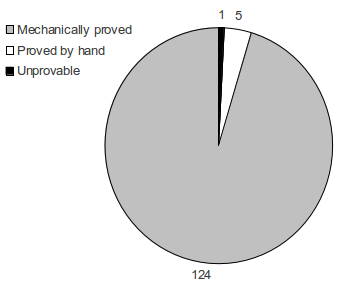
\includegraphics[width=\textwidth]{proverEval/proofResults.png}
		\caption{Number of Search Steps Required by VC\label{fig:pie}}
	\end{subfigure}
	\begin{subfigure}[b]{0.55\textwidth}
		\centering
		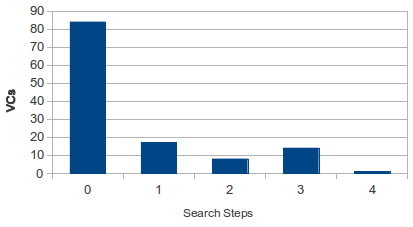
\includegraphics[width=\textwidth]{proverEval/searchSteps.png}
		\caption{Number of Search Steps Required by Proofs\label{fig:histogram}}
	\end{subfigure}
	\caption{Summary of Proof Evaluation Results}
\end{figure}

As we have previously mentioned, we are particularly interested in the search step metric since it represents the only non-deterministic portion of the proof search.  That the median number of such steps was zero is extremely heartening and we are further encouraged that no VC required more than four.  Figure \ref{fig:histogram} shows a histogram of the number of VCs requiring different numbers of search steps.

The vast majority (84, or 68\%) of VCs required no search steps once all heuristics were applied.  39 (31\%) required three or fewer steps, while only a single VC required four search steps.  This data supports our hypothesis that VCs arising from well-engineered software should require only simple analysis to dispatch.
